\chapter{Methods and Materials}
\section{Wastewater treatment plant description}
\subsection{Process and data sources in SWHEPP}
Shek Wu Hui Effluent Polish Plant (SWHEPP) is a secondary sewage treatment plant, which treats the municipal wastewater of the Sheung Shui, Fanling Districts and adjacent areas, and treated leachate effluent from North East New Territories (NENT) leachate treatment plant. The plant is designed for 300,000 population equivalents (PE) in 2001, and in 2009, the daily treatment capacity has been expanded from 80,000 m$^3$/day to 93,000 m$^3$/day. SHWEPP is operated and maintained by Drainage Services Department (DSD), and the plant will be upgraded to teritary treatment level to increase the treatment capacity of 190,000 m$^3$/day by the end of 2025. As shown in Fig.~\ref{fig:SHWEPP-flowchart}, the treatment plant is mainly comprised of primary sedimentation, secondary biological treatment, and final sedimentation followed by a membrane bioreactor (MBR), which provides an advanced level of organic and suspended solids removal. To monitor the effluent quality in real-time, low volume of the MBR effluent is pumped to an effluent container near by the MBR location. Two on-line meters, ammoniacal nitrogen on-line sensor and colour level on-line analyzer are installed in the effluent container, which are indicated as (a) and (b) in Fig.~\ref{fig:SHWEPP-flowchart}.

\begin{figure}[h]
    \centering
    \includegraphics[width=0.9\columnwidth]{imgs/Sewage-treatment-process-flowchart.png}
    \caption{Sewage treatment process flowchart at SWHEPP (adapted from Drainage Services Department 2020)}
    \label{fig:SHWEPP-flowchart}
\end{figure}

\section{Data collection and preparation}

\begin{figure}[h]
    \centering
    \includegraphics[width=0.8\columnwidth]{imgs/instrument/sampling-tank.png}
    \caption{Colour levels and ammonia concentration are measure in the effluent container (i.e., on the right of the image.) A water pump transports MBR effluent to the effluent container continuously at real-time. The black vault on the left of the image contains a laptop and a colour spectrophotometer.} 
    \label{fig:sampling-tank}
 \end{figure}

\subsection{On-line data monitoring and collection}
To enable us to perform on-line monitoring of ammonium concentration (NH$_{3}$-N) in the MBR effluent, a Ammonium and Potassium Probe, AmmoLyt$^\circledR$Plus 700 IQ (Xylem Company) is installed as in Fig.~\ref{fig:nh3-sensor-a} in the effluent container, as shown in Fig.~\ref{fig:sampling-tank}. The operation was commenced on 27 April 2021 and completed on 27 March 2022. The ion-selective electrode (ISE) probe provides continuous and reagentless monitoring of ammonium and potassium at the configured interval of one measurement per minute. Due to the ISE probe cannot differentiate the potentials difference cause by ammonium and potassium ions in the electrodes, the on-line monitoring of ammonium concentration requires the continuous calibration using potassium concentration.

The instrument records ammonium concentration as NH$_{4}$-N mg/L, a form to express the sum of nitrogen found in reduced nitrogen (III) form. Ammonia has a reported pKa of 9.25 \citep{nationalcenterforbiotechnologyinformationPubChemCompoundSummary2022}, meaning ammonium is a primary species under the pH of 9.25 in water. In WWTPs, the pH in water normally ranges from pH of 7--8, making the NH$_{4}$-N concentration the dominant species. Both ammonia and ammonium contain one nitrogen atom, 1 mg/L NH$_{3}$-N is the same as 1 mg/L NH$_{4}$-N. Thus, to prevent confusion, in the following paragraph the unit of NH$_{4}$-N will be expressed by NH$_{3}$-N, which is the unit used in the water quality standard. The collection of on-line ammonia data is achieved through downloading csv files from the website connected to the IQ Sensor Controller (Xylem Comapny), as shown in Fig.~\ref{fig:nh3-sensor-b}. 

\begin{figure}[h]
    \centering
    \begin{subfigure}{0.3\textwidth}
      \includegraphics[width=\linewidth]{imgs/instrument/ammonium-sensor.png}
      \caption{AmmoLyt$^\circledR$Plus 700 IQ, Xylem} \label{fig:nh3-sensor-a}
    \end{subfigure}%
    \hspace{5em}%   % maximize separation between the subfigures
    \begin{subfigure}{0.3\textwidth}
      \includegraphics[width=\linewidth]{imgs/instrument/controller-for-iq-sensor.png}
      \caption{DIQ/S 284-EF controller, Xylem} \label{fig:nh3-sensor-b}
    \end{subfigure}%  
  \caption{Instrument of on-line ammonium monitoring system.} \label{fig:nh3-sensor}
\end{figure}

An hourly monitoring of the colour levels of MBR effluent was conducted from 5 October 2021 to 26 February 2022 by using a custom-made on-line colour analysis system. Originally, the spectrophotometer as Fig.~\ref{fig:hach-sip} and a peristaltic pump as Fig.~\ref{fig:hach-dr3900} can only initiate a single measurement of colour level by pressing the "READ" buttom on the DR3900 panel. To realize continuously sampling and analyzing colour level without human intervention, an actuator with programmable time function was mounted on the panel of DR3900, as shown in Fig.~\ref{fig:hach-actuator}. 

The automatic sampling and analzying of the colour level begins with the action of the actuator, by clicking on the "READ" button to initiate the colour analysis at a fixed interval of 30 minutes. 3 mL of sample was collected from the effluent container and delivered to the spectrophotometer cell. Then, the sample was subsequentially analysed by the spectrophotometer with the data transmitted to an automatic data acquisition and storage software pre-installed in the laptop. The DR3900 device is connected to a laptop, which receives the real-time data and stores on a data management software from Hach company. To access the real-time data from the laptop, Google Remote Desktop is used to operate the laptop via Internet cloud services using any devices having access to the Internet. The entire process is illustrated in Fig.~\ref{fig:diagram-colour-analysis}. After the measurement, the sample will be discharged to the effluent container and the online colour monitoring system is left idle until the next measurement. 

\begin{figure}[h]
    \centering
    \begin{subfigure}{0.3\textwidth}
      \includegraphics[width=\linewidth]{imgs/instrument/SIP10.png}
      \caption{SIP10 peristaltic pump, Hach} \label{fig:hach-sip}
    \end{subfigure}%
    \hspace{2em}   % maximize separation between the subfigures
    \begin{subfigure}{0.3\textwidth}
      \includegraphics[width=\linewidth]{imgs/instrument/DR3900_PS.png}
      \caption{DR3900 spectrophotometer, Hach} \label{fig:hach-dr3900}
    \end{subfigure}%
    \vspace{2em}
    \begin{subfigure}{0.7\textwidth}
        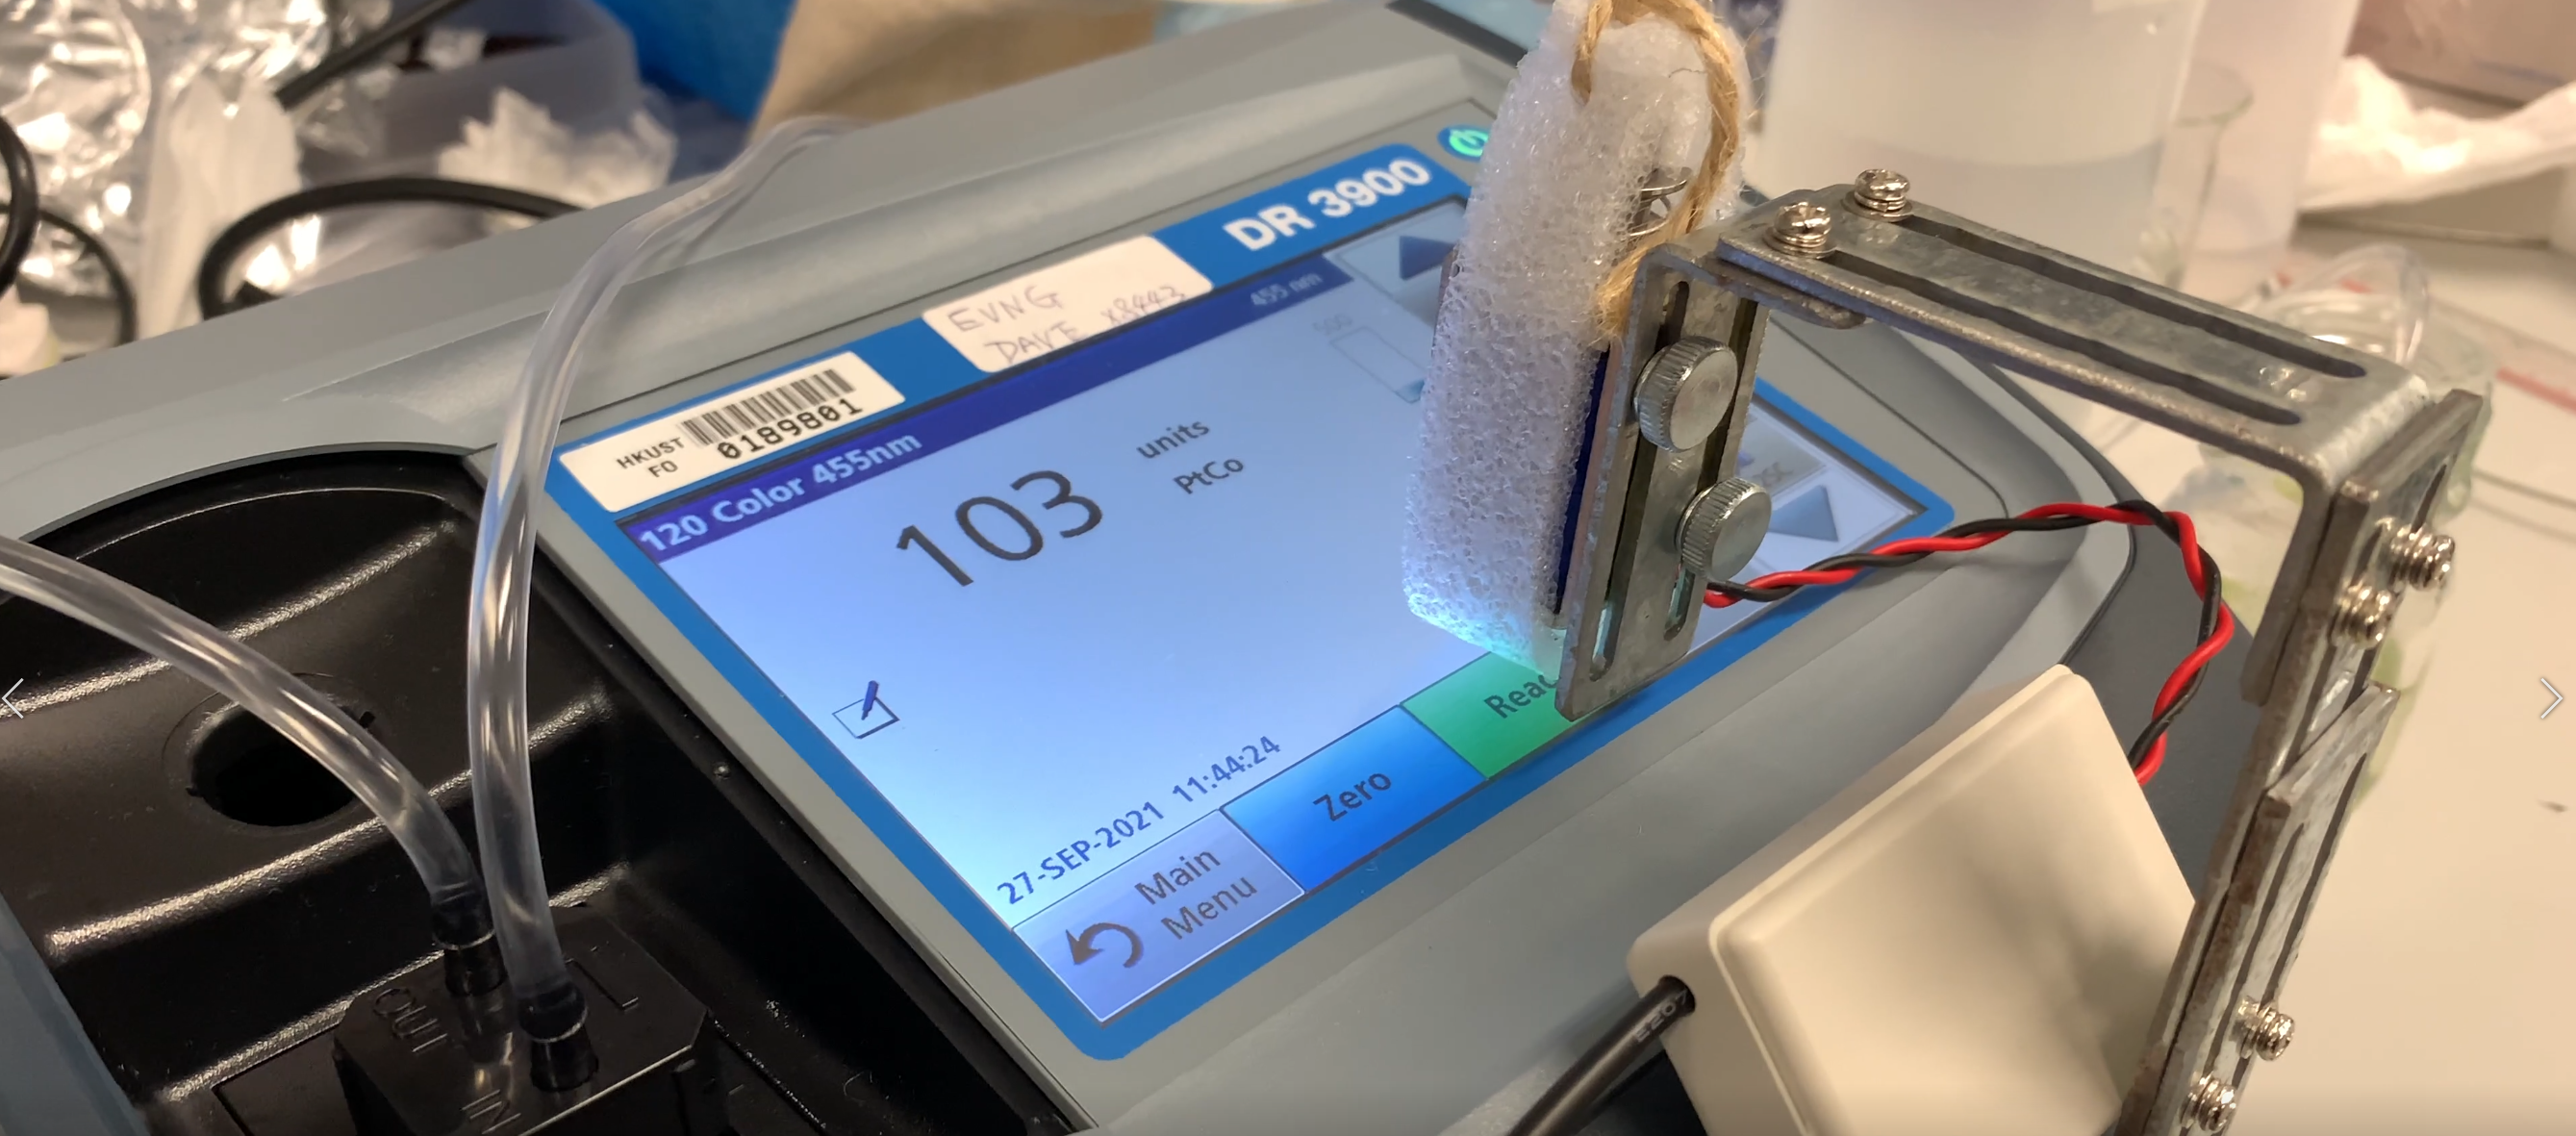
\includegraphics[width=\linewidth]{imgs/instrument/actuator-mount.png}
        \caption{Customized clicker/actuator} \label{fig:hach-actuator}
    \end{subfigure}%  
  \caption{Instruments of on-line colour analysis system.} \label{fig:hach}
\end{figure}

The maintenance and calibration of the DR3900 spectrophotometer is performed on a weekly basis. During the maintenance, the DR3900 device was shut off, and chlorine solution at the concentration of 100 mg/L was pumped into the sampling tubes and the plastic cuvette for disinfection and cleansing. The cleanse of the tubes and cuvette were manually inspected with eyes to make sure no foreign objects were stuck inside. De-ionized water was brought to the site to perform the spectrophotometer calibration after the reboot of DR3900. 

\begin{figure}[h]
    \centering
    \includegraphics[width=0.8\columnwidth]{imgs/instrument/colour-sampler.png}
    \caption{Schematic diagram of the custom-made on-line colour anlaysis system.}
    \label{fig:diagram-colour-analysis}
 \end{figure}

\subsection{Loss function for model evaluation}
Loss functions are used to determine the error between the model outputs (i.e., prediction or forecasting values) and the given target value \citep{deepaiLossFunction2022}. The bigger the difference between the ground truth $\bm{y}$ and the model outputs $\bm{\hat{y}}$, the higher the value of the loss function is, meaning the model perfomred poorer. A low value for the loss means the modle perfomred well. The selection of the types of the loss function is essential for training the model to perform specific tasks. In this study, Mean Squared Error (MSE) is used for evaluating the regression models. The values of MSE will never be negative, and is formally defined by the following equation:

\begin{equation}\label{eq-mse}
    MSE=\frac{\sum (y_i-\hat{y_i})^2}{n}
\end{equation}

\subsection{Data cleaning and pre-processing}
In this study, ammonia concentration and colour level forecasting models will be trained, and the model training steps are shown in Fig.~\ref{fig:training-scheme}. The training processes are split into two sections, one is the baseline model training steps, the other is proposed model training steps. The training steps of the first section used cleaned data to train forecasting models and generated baseline model performance, which will be further compared with the model perfromance generated from the second section. The second section includes using pre-processed datasets (i.e., data smoothing) and feature engineering enhanced datasets to train the forecasting model. In machine learning, the data used for training models is refered to model inputs, features and variables.

\begin{figure}[h]
    \centering
    \includegraphics[width=0.9\columnwidth]{imgs/pre-processing/training-scheme.png}
    \caption{Machine learning model training steps.}
    \label{fig:training-scheme}
\end{figure}

The raw data embedded in the original csv files exists many issues, such as missing values, having extreme low or high values, and unreadable texts, etc. Thus, the data cleaning and pre-processing are necessary for more effective process of model training. Python programming language and related modules of Numpy and Pandas were used to clean and pre-process the raw dataset for further usage. The ammonia raw dataset contained 44,640 samples (data points) with 8 variables, giving a matrix size of 44,640 x 8, and the samples were collected in time series at 1 minute interval. The colour level raw dataset contained 1488 samples with 34 variables, giving a matrix size of 1488 x 34, and the samples were collected in time series at 30 minute interval.

Before the high-resolution data from colour and ammonia datasets were compressed into time series data at 1 hour interval via averaging, extreme values were manually removed. For ammonia dataset, we replaced the values higher than 7.0 mg/L with NaN (i.e., Not a number), and futher use interpolation to fill up the NaN along with the missing values in the dataset. For colour dataset, we manually took out the relatively low data points on the days when the maintenance and calibration tasks were performed; extremely values higher than 300 Hazen Unit were also replaced by NaN. Same as the data cleaning method used for ammonia dataset, the missing values and NaN were filled up via interpolation.

\subsubsection{Data smoothing with Savitzky-Golay and EWMA filter}
Data smoothing was performed on both ammonia and colour datasets using the same method. One of the effective ways to remove the noise from the dataset is to apply data smoothing filters. Two filteres were applied in this study, Savitzky-Golay (SG) and Exponentially Weighted Moving Average (EWMA) filters.

A SG filter is a digital filter that can be applied to a set of digital data points for the purpose of smoothing the data without distorting the data tendency. This is achieved via convolution, by fitting successive sub-sets of adjacent data points with a low-degree polynomial by the method of linear least squares \citep{wikipediaSavitzkyGolayFilter2022}. The illustration is shown in Fig.~\ref{fig:filters-sg} and the procedures of how data points are smoothed is presented in the following steps:

\noindent
\begin{myenumerate}
    \item Extract short-time window (i.e., blue dots in Fig.\ref{fig:filters-sg})
    \item Determine polynomial degree (e.g., different polynomial degree is compared in Fig.~\ref{fig:filters-sg}).
    \item Find the smoothed data point (i.e., at center of the window).
    \item Repeat for shifted window (e.g., similar to moving average).
\end{myenumerate}

The equation to decribed the smoothed value of $\bm{Y_j}$ can be expressed in Eq.~\ref{sg-eq}:

\begin{equation}\label{sg-eq}
    Y_j=(C\otimes y)_j=\sum_{i=\frac{1-m}{2}}^{\frac{m-1}{2}}C_iy_{j+i},\,\frac{m+1}{2}\le j\le n-\frac{m-1}{2}
\end{equation}

\noindent
where $Y_j$ corresponds to the $j^{th}$ smoothed data point, $m$ to the window size (i.e., numer of data points intended to smooth out) and $C_i$ to the convolution coefficients (i.e., determined by \citet{savitzkySmoothingDifferentiationData1964}). 

Exponentially weighted moving average (EWMA), also known as auto-regressive (AR) filtering, is a technique that filters measurements. An EWMA filter smoothes a measured data point by exponentially averaging that particular point with all previous measurements. The EWMA equation can be expressed in Eq.~\ref{ewma-eq}:

\begin{equation}\label{ewma-eq}
    \begin{aligned}
        &\alpha=\frac{2}{span+1} \\
        &y_0=x_0 \\
        &y_t=(1-\alpha)y_{t-1}+\alpha x_t
    \end{aligned}
\end{equation}

\noindent
where $\alpha$ corresponds to the decay paratmeter, $x_t$ to the value at a time period, $y_t$ to the value of the EWMA at any time period t, span to the window size.

\begin{figure}[h]
    \centering
    \begin{subfigure}[t]{0.4\textwidth}
      \includegraphics[width=\linewidth]{imgs/pre-processing/demo-polynomial-fitting.png}
      \caption{SG filter with different polynomial degree \citep{taalSmoothingYourData2017}.} \label{fig:filters-sg}
    \end{subfigure}%
    \hspace{2em}%   % maximize separation between the subfigures
    \begin{subfigure}[t]{0.5\textwidth}
      \includegraphics[width=\linewidth]{imgs/pre-processing/demo-weight-ewma.png}
      \caption{Examples of weights with exponential decay at varied alpha values \citep{cfiExponentiallyWeightedMoving2022}.} \label{fig:filters-ewma}
    \end{subfigure}%  
  \caption{Illustration of the influence of different polynomial degrees in the fitting of SG filter and the weigth decay with varied alpha values in EWMA filter.} \label{fig:filters}
\end{figure}

Both SG and EWMA filters are required to select the hyperparamters, the selected values are presented in Table.~\ref{tab:filter-hyperparameters}.

\begin{table}[!ht]
    \centering
    \caption{The selected hyperparameters for SG and EWMA filters.}\label{tab:filter-hyperparameters}
    \begin{NiceTabular}{lcc}
        \toprule
        Group Name & Window size & Polynomial degree \\
        \midrule
        SG-5   & 5 & 2 \\ 
        SG-7   & 7 & 2 \\ 
        SG-9   & 9 & 2 \\ 
        EWMA-2 & 2 & - \\ 
        EWMA-3 & 3 & - \\ 
        EWMA-4 & 4 & - \\ 
        \bottomrule
    \end{NiceTabular}
\end{table}

\subsubsection{Outlier Removal}
Despite the extreme values in the ammonia raw dataset were removed based on simple conditions (i.e., concentration higher than 7.0 mg/L), the ammonia sensor can still capture unideal data points collectively. In the outlier removal process, we intended to identify the collective faults of ammonia data in the unit of an entire day. To determine whether the ammonia data on a specific day shows collective fault, two abnormal conditions are defined:

\noindent
\begin{myenumerate}
    \item NH$_{3}$-N fluctuation $\le$ 0.1 (i.e., lower than the sensor resolution).
    \item No diurnal fluctuation (i.e., Fluctuation = peak value – bottom line value).
\end{myenumerate}

To automiatically realize the identification of noraml or abnormal signals, peak analysis was performed on the daily ammonia data. The analysis takes a one-dimension array (i.e., the data form of ammonia in a day) and finds all local maximum values by simple comparison of neighboring values. This function will also provide information such as width and prominence, as in Fig.~\ref{fig:prominence} to help us identify whether the diurnal fluctuation is existed.

\begin{figure}[h]
    \centering
    \includegraphics[width=0.55\columnwidth]{imgs/pre-processing/prominence.png}
    \caption{Illustration of peak analysis. Four important elements are automatic caculated by the function \citep{mathworksDocumentationFindpeaks2022}.}
    \label{fig:prominence}
 \end{figure}

\subsubsection{Feature Engineering}
To create addition features from the raw datasets, we have carefully observed and analyzed the SWHEPP influent. We discovered that the SWHEPP influent is consisted of treated landfill effluent from NENT landfill leachate site and municipal wastewater, as shown in Fig.~\ref{fig:geomap}. Treated leachate effluent mainly contributes the colour levels in the SHWEPP influent, while the ammonia concentration is mostly from the municipal wastewater. During the mixing of both type of the wastewater as in Fig.~\ref{fig:blend-ratio}, pollutants contribute to colour levels will be diluted by the municipal wastewater, same as the opposite for the dilution of ammonia concentration. The changes of colour levels and ammonia concentration are related, thus, in feature engineering, colour level data was selected for training ammonia forecasting model; ammonia data was selected for training colour forecasting model, as shown in Fig.~\ref{fig:feature-selection}.

\begin{figure}[h]
    \centering
    \includegraphics[width=0.95\columnwidth]{imgs/pre-processing/geomap.png}
    \caption{Sewer system coverage of SHWEPP. The covered areas (i.e., area circled in red boundary) include Fanling/Sheung-Shui new towns and NENT landfill leachate treament plant.}
    \label{fig:geomap}
 \end{figure}

\begin{figure}[h]
    \centering
    \begin{subfigure}[t]{0.45\textwidth}
      \includegraphics[width=\linewidth]{imgs/pre-processing/blending-ratio.png}
      \caption{Flowchart showing the blending of treated leachate effluent with municipal wastewater.} \label{fig:blend-ratio}
    \end{subfigure}%
    \hspace{2em}%   % maximize separation between the subfigures
    \begin{subfigure}[t]{0.45\textwidth}
      \includegraphics[width=\linewidth]{imgs/pre-processing/pos-encoding.png}
      \caption{Positional encoding of hour components.} \label{fig:pos-encoding}
    \end{subfigure}%  
  \caption{Analysis of influent quality composition and the illustration of the positional encoding.} \label{fig:blend-pos}
\end{figure}

\begin{figure}[h]
  \centering
  \includegraphics[width=0.8\columnwidth]{imgs/results/colour-pattern.png}
  \caption{}
  \label{fig:color-to-nh3-pattern}
\end{figure}

\begin{figure}[h]
  \centering
  \includegraphics[width=0.8\columnwidth]{imgs/leachate-effluent-blend-ratio-color-plot/colour-blend-coef.png}
  \caption{}
  \label{fig:blend-colour-coef}
\end{figure}

The new features are inspired from the research work of \citet{abu-bakarQuantifyingImpactCOVID192021}. The author pointed out the four types of hourly household water consumption patterns as in Fig.~\ref{fig:water-consumption-pattern}, which correlates the specific time of the day to the volume of the water consumed in households. In other words, as fresh water is consumed, wastewater is generated at the same time, the wastewater then enters the public sewage system and result in the increase of ammonia concentration. Thus, it is convinced that time features will be able to help the machine learning models to better correlate and predict the change of ammonia concentration in the wastewater. 

Time feature is realized through a technique called positional encoding (POS). The positioanl encoded feature was achieved as the following steps:

\noindent
\begin{myenumerate}
    \item The timestamp are represented as three elements---hour, day and month.
    \item Each element will bed decomposed into sine and cosine components.
    \item Last step is applied to hours and days to make all elements represented cyclically.
\end{myenumerate}

Due to the size of the datasets used in this study for training ammonia and colour forecasting model is 31 days, only hour element was transformed into sine and cosine components as in Fig.~\ref{fig:pos-encoding}.

\begin{figure}[h]
    \centering
    \includegraphics[width=0.8\columnwidth]{imgs/pre-processing/hourly-consumption-pattern.png}
    \caption{Hourly water consumption patterns in households \citep{abu-bakarQuantifyingImpactCOVID192021}. (a) Cumulative pattern and percentage of hourly consumption for households in the “Evening Peak (EP)” cluster (b) Cumulative pattern and percentage of hourly consumption for households in the “Late Morning Peak Peak (LM)” cluster. (c) Cumulative pattern and percentage of hourly consumption for households in the “Early Morning Peak (EM)” cluster. (d) Cummulative pattern and percentage of hourly consumption for households in the “Multiple Peak (MP)” cluster. Consumption is in (m3).}
    \label{fig:water-consumption-pattern}
 \end{figure}

\begin{figure}[h]
  \centering
  \includegraphics[width=0.8\columnwidth]{imgs/results/nh3-pattern.png}
  \caption{The daily patterns of ammonia concentration on 3, 7, 11, 15 Janurary 2022.}
  \label{fig:nh3-peak-pattern}
\end{figure}

\subsection{Data transformation}
Before the pre-processed data is fed into the models for training, we need to split the data into three clusters, which are training (60\%), validation (20\%), and testing dataset (20\%). Among each training dataset, the data will be further split into input variables $\bm{X}$ and output variable $\bm{Y}$ (i.e., training X/training Y, testing X/testing Y). During the training process, machine learning algorithms will learn a target function $\bm{f}$ to best map $\bm{X}$ to $\bm{Y}$. 

A taining dataset is a set of examples (e.g., historical data) for models to learn the hidden trends and information in the data, shown in (a) in Fig.~\ref{fig:training-scheme}, and the training loss is calculated by taking the sum of loss for each example in the training dataset after each epoch. Since it is impossible to have the optimized hyperparameters in the first try of the training, a validation dataset as in (b) in Fig.~\ref{fig:training-scheme} is used to assess the model performance until we obtain the optimzed settings. The validation loss plays an important role during the model training, the adjustments of the hyperparameters will directly reflect on the change of the validation loss, the lower the values, the better the model performance is. As the optimzed model is obtained, testing dataset is used to evaluate the performance of the forecasting model, as shown in (c) in Fig.~\ref{fig:training-scheme}. To the forecasting Models, testing dataset has never been seen by the models. If the model tuning process was performed on the testing dataset, the model performance would be a biased result since the hyperparameters are revised in favor to the evalution of the testing dataset.

In Fig.~\ref{fig:training-scheme}, the hyperparameters will remained the same once the optimzed values are found, thus generating a baseline model perfromance of a specific machine learning model. The baseline results will be further compared with the results from the model trained by the proposed model trianing steps, which include datasets that have been performed data smoothing and feature engineering techniques.

\begin{figure}[h]
    \centering
    \includegraphics[width=0.8\columnwidth]{imgs/pre-processing/feature-selection.png}
    \caption{Illustration of feature selections for model training.}
    \label{fig:feature-selection}
 \end{figure}

\section{Machine learning models}
\subsection{Random Forest}
The machine learning model used in this study (i.e., not deep learning models) is random forest (RF). It is an ensemble method which the final output is obtained by averaging the results from multiple tree learners \citep{wangMachineLearningFramework2021}, as shown in Fig.~\ref{fig:rf}. The training algorithm applies the general technique of bootstrap aggregating, also known as bagging, to tree learners. Given a training set $X = x_1, ..., x_n$ with targets $Y = y_1, ..., y_n$, bagging repeatedly (B times) selects a random sample with replacement (i.e., not putting the samples back to the population) of the training set and fits trees to these samples \citep{wikipediaRandomForest2022}, RF generate an output through the following steps:

For $b=1, ..., B:$

\noindent
\begin{myenumerate}
  \item Sample (with replacement) n training examples from $X$, $Y$, call these $X_b, Y_b$.
  \item Train a regression tree $f_b$ on $X_b, Y_b$.
  \item Predict unseen samples $x^{'}$ by averaging the predicdtions from all the regression tree learners on $x^{'}$ as in Eq.~\ref{eq-rf}:
\end{myenumerate}

\begin{equation}\label{eq-rf}
  \hat{f}=\frac{1}{B}\sum_{b=1}^{B}f_b(x^{'})
\end{equation}

\subsection{Deep Neural Networks}
Artificial Neural Network (ANN) is a very broad term that encompasses any form of Deep Learning model. A typical ANN consists with input, hidden and output layers, and each layer comprises multiple neurons (i.e., nodes). The connected neurons are to simulate the human brain by process and transmit input signals to the next nodes \citep{mohseni-dargahChapter12Machine2022} . What sets apart from a ANN model to a DNN model is that the former contains only one hidden layer while the latter has more than one, as shown in Fig.~\ref{fig:dnn}. The DNN models are nonlinear, which finds the correct mathematical manipulation to turn the input into the output \citep{bangaloreaiDeepNeuralNetwork2018}.

\begin{figure}[h]
  \centering
  \begin{subfigure}[t]{0.5\textwidth}
    \includegraphics[width=\linewidth]{imgs/models/random-forest.png}
    \caption{Random Forest (RF) \citep{riebesellRandomForest2022}.} \label{fig:rf}
  \end{subfigure}%
  \hspace{3em}%   % maximize separation between the subfigures
  \begin{subfigure}[t]{0.4\textwidth}
      \includegraphics[width=\linewidth]{imgs/models/DNN.png}
      \caption{Deep Neural Network (DNN) \citep{ibmNeuralNetworks2022}.} \label{fig:dnn}
  \end{subfigure}%
\caption{Illustration of RF and DNN model structure.} \label{fig:rf-dnn}
\end{figure}

%An ANN is based on a collection of connected units or nodes called artificial neurons, which loosely model the neurons in a biological brain. Each connection, like the synapses in a biological brain, can transmit a signal to other neurons. An artificial neuron receives signals then processes them and can signal neurons connected to it. The "signal" at a connection is a real number, and the output of each neuron is computed by some non-linear function of the sum of its inputs. The connections are called edges. Neurons and edges typically have a weight that adjusts as learning proceeds. The weight increases or decreases the strength of the signal at a connection. Neurons may have a threshold such that a signal is sent only if the aggregate signal crosses that threshold. Typically, neurons are aggregated into layers. Different layers may perform different transformations on their inputs. Signals travel from the first layer (the input layer), to the last layer (the output layer), possibly after traversing the layers multiple times.

\subsection{Recurrent Neural Network}
A recurrent neural network (RNN) is a type of Artificial Neural Network which designed to work with sequence data. For instance, sequence data are time series, DNA, language, speech and sequences of user actions data, etc. The ammonia concentration and colour level data are time series data, which is a series of data points listed in minute orders \citep{dongesGuideRNNUnderstanding2021}. A distinguished characteristic of RNN is that they share parameters across each layer of the network by allowing information to be passed from last step of the network to the next. Unlike RNN, feedforward networks like DNN have different weights across each node. The reuse of previous information for making decision on RNN makes it capable of "learning" from the previous inputs. The realization of the memorizing function is through a memory unit called hidden state (i.e., a vector contains weights) in RNN architecture, which enable RNN to presist data, thus capture short term dependencies. The RNN architecture is presented in Fig.~\ref{fig:rnn}. The general formulation of a RNN is expressed in Eq.~\ref{eq-rnn} \citep{mamandipoorMonitoringDetectingFaults2020}:

\begin{equation}\label{eq-rnn}
  h_t=\sigma(W^hh_{t-1}+W^xx_t+b)
\end{equation}

\noindent
where $x_t$ is the current input, $h_t$ is the current hidden state (output), $h_{t-1}$ is the previous output, $W^x$ is the weights of the hidden state, $W^h$ is the weight of the input, $b$ is the bias, $\sigma$ is the sigmoid activation function.

\begin{figure}[h]
    \centering
    \begin{subfigure}[t]{0.3\textwidth}
      \includegraphics[width=\linewidth]{imgs/models/rnn-2.png}
      \caption{Recurrent Neural Network (RNN).} \label{fig:rnn}
    \end{subfigure}%
    \hspace{1em}%   % maximize separation between the subfigures
    \begin{subfigure}[t]{0.3\textwidth}
      \includegraphics[width=\linewidth]{imgs/models/lstm-2.png}
      \caption{Long Short-term Memory (LSTM).} \label{fig:lstm}
    \end{subfigure}%
    \hspace{1em}
    \begin{subfigure}[t]{0.3\textwidth}
      \includegraphics[width=\linewidth]{imgs/models/gru-2.png}
      \caption{Gate Recurrent Unit (GRU).} \label{fig:gru}
    \end{subfigure}%  
  \caption{Variant architectures of Recurrent Neural Networks (adapted from \citet{olahUnderstandingLSTMNetworks2015}).  $x_t$ corresponds to the current input, $h_{t-1}$ to the last hidden state (output), $h_t$ to the current output, tanh is the tangent activation function, $\sigma$ is the sigmoid activation function,$\times$ is the vector pointwise multiplication, $+$ is the vector pointwise addition.} \label{fig:recurrent-nn}
\end{figure}

\subsection{Long Short-term Memory}
Long Short-term Memory (LSTM) is a deep recurrent neural networks (RNN), an advanced and improved version of RNN. The advent of LSTM is to solve problems requiring learning long-term temporal dependencies which cannot be learned by RNN due to the simple model architecture. The fundmental of LSTM network is built on memory blocks called "cells", which are responsible for tranferring and receiving the states (i.e., vectors) recording the information from the previous cells. In a cell block, there are input gate, forget gate and the output gate. The function of these three gates is to control the movement of the information into and out of the cell via the sigmoid function. The inputs of the cell will first go through a forget gate ($f_t$) as Eq.~\ref{lstm-(1)}, where the function will mutiply each element in the input states by values ranging from 0 to 1 to realize the effect of "forget". Next, a input gate ($i_t$) as in Eq.~\ref{lstm-(2)} will decide whether the new information should be updated or ignored by sigmoid function (i.e., 0 or 1), followed by a tangent function giving weight of importance (i.e., -1 to 1) to the values which passed by as in Eq.~\ref{lstm-(3)}. New memory then is appended to the previous memory $C_{t-1}$ resulting a new $C_t$. Lastly, output values ($h_t$) is obtained based on output cell state ($O_t$) as in Eq.~\ref{lstm-(5)} and Eq.~\ref{lstm-(6)} \citep{leApplicationLongShortTerm2019}. The equations for LSTM structure are shown in Eq.~\ref{eq-lstm}:

\begin{subequations} \label{eq-lstm}
  \begin{align}
      &f_t=\sigma(W_f[h_{t-1},X_t]+b_f) \label{lstm-(1)}\\
      &i_t=\sigma(W_i[h_{t-1},X_t]+b_i) \label{lstm-(2)}\\
      &\tilde{C_t}=tanh(W_n[h_{t-1},X_t]+b_n) \label{lstm-(3)}\\
      &C_t=C_{t-1}f_t+\tilde{C_t}i_t \label{lstm-(4)}\\
      &O_t=\sigma(W_o[h_{t-1},X_t]+b_o) \label{lstm-(5)}\\
      &h_t=O_ttanh(C_t) \label{lstm-(6)}
  \end{align}
\end{subequations}

\noindent
where $f_t$ corresponds to the forget gate, $i_t$ to the input gate, $\tilde{C_t}$ to the candidate cell state, $C_t$ to the current cell state, $O_t$ to the output cell state, $h_t$ to the output values, $\sigma$ to the sigmoid function, $X_t$ to the current input, tanh to the tangent function, $W$ and $b$ are the weight matrices and bias of the corresponding output gate, respectively.

\subsection{Gate Recurrent Unit}
Gated Recurrent Unit (GRU) model is a variant of LSTM model, by combining the forget gate and input gate into an update gate as in Fig.~\ref{fig:gru}, GRU has less parameters compared to LSTM. The advantage of GRU over LSTM is less computing power required while maintaining a similar model performance compared to LSTM. The inputs of GRU model first enter the update gate ($z_t$) as in Eq.~\ref{gru-(1)}, where the function will help the model to determine how much of the past information needs to be passed along to the future via sigmoid functions. Followed by the reset gate ($r_t$) as in Eq.~\ref{gru-(2)}, which is used to decide how much of the past information to forget. Althogh Eq.~\ref{gru-(1)} and Eq.~\ref{gru-(2)} have the same inputs of $X_t$ and $h_{t-1}$, the usages of the gates are different. The outputs of reset gate will be used to determine the candidate hidden state ($]tilde{h}$) as in Eq.~\ref{gru-(3)}, where the tangent fucntion will determine the importance of current input ($X_t$), reset gate output, and previous hidden state ($h_t$). At the last step, the output values ($h_t$) is calculated from the candidate hidden state ($\tilde{h_t}$), previous hidden state ($h_{t-1}$), and the outputs of update gate as in Eq.~\ref{gru-(4)}. The equations of GRU structures are presented in Eq.~\ref{eq-gru} \citep{chengForecastingWastewaterTreatment2020}:

\begin{subequations} \label{eq-gru}
  \begin{align}
      &z_t=\sigma(X_tW_{xz}+h_{t-1}W_{hz}+b_z) \label{gru-(1)}\\
      &r_t=\sigma(X_tW_{xr}+h_{t-1}W_{hr}+b_r) \label{gru-(2)}\\
      &\tilde{h_t}=tanh(X_tW_{xh}+(r_t\circ h_{t-1})W_{hh}+b_h) \label{gru-(3)}\\
      &h_t=z_t\circ h_{t-1}+(1-z_t)\circ \tilde{h_t} \label{gru-(4)}
  \end{align}
\end{subequations}

\noindent
where $z_t$ corresponds to the update gate, $r_t$ to the reset gate, $\tilde{h_t}$ to the candidate hidden state, $h_t$ to the output values, $\sigma$ to the sigmoid function, tanh to the tangent function, $X_t$ to the current input, $W$ and the $b$ are the weight matrices and bias of the corresponding output gate, respectively.

%\section{Implementation of regularization}
%\subsection{Scheduler}